\documentclass[12pt,a4paper]{article}

\usepackage[utf8]{inputenc}
\usepackage[T1]{fontenc}
\usepackage{lmodern}
\usepackage[margin=2.5cm]{geometry}
\usepackage{amsmath,amssymb,amsthm}
\usepackage{booktabs}
\usepackage{tabularx}
\usepackage{graphicx}
\usepackage{tikz}
\usepackage{listings}
\usepackage{xcolor}
\usepackage{enumitem}
\usepackage[hidelinks]{hyperref}
\usepackage{url}

% ---------------------------------------------------------------------------
% Fill in before submitting
% ---------------------------------------------------------------------------
\newcommand{\studentid}{\textcolor{red}{ID}}
\newcommand{\supervisor}{\textcolor{red}{Supervisor name}}

% ---------------------------------------------------------------------------
% Notation
% ---------------------------------------------------------------------------
\newcommand{\T}{\mathcal{T}}
\newcommand{\Colorer}{\mathit{Colorer}}
\newcommand{\AllDiff}{\mathit{AllDifferent}}
\newcommand{\Enc}{\mathit{Enc}}
\newcommand{\tool}{\textsc{KColor}}
\newcommand{\enc}[1]{\texttt{#1}}

\newtheorem{definition}{Definition}
\newtheorem{theorem}{Theorem}
\newtheorem{lemma}{Lemma}
\newtheorem{property}{Property}
\theoremstyle{definition}
\newtheorem{example}{Example}

\lstset{
  basicstyle=\ttfamily\small,
  columns=fullflexible,
  keepspaces=true,
  frame=single,
  framesep=4pt,
  xleftmargin=6pt,
  xrightmargin=6pt,
  commentstyle=\color{gray},
  morecomment=[l]{;},
}

\usetikzlibrary{positioning}
\tikzset{
  vertex/.style={circle, draw, thick, minimum size=7mm, inner sep=0pt, font=\small},
}

\begin{document}

% ---------------------------------------------------------------------------
% Title page
% ---------------------------------------------------------------------------
\begin{titlepage}
  \centering
  {\Large Bar Ilan University\par}
  \vspace{0.6cm}
  {\large Computer Science Department\par}
  {\large M.Sc Proposal\par}
  \vspace{3cm}
  {\huge\bfseries Graph Coloring Modulo Theories\par}
  \vspace{0.5cm}
  {\Large Colorers, Encodings and Solvers\par}
  \vspace{3cm}
  {\large Author:\par}
  {\large Omer Silberman (213973795)\par}
  \vspace{1.5cm}
  {\large Supervisor:\par}
  {\large Dr. Yoni Zohar\par}
  \vfill
  {\large \today\par}
\end{titlepage}

% ===========================================================================
\section{Introduction}
% ===========================================================================

Satisfiability Modulo Theories (SMT) is a prominent research direction in
verification. SMT generalizes the Boolean satisfiability problem, known as SAT,
and supports first-order logic and theories. For example, important first-order
theories are integers, real numbers, arrays, strings, bit-vectors, and
more~\cite{BarrettST10,ZhengZG13,ReynoldsB16}. The task of SMT-solvers is to read a
formula in first-order logic with some background theory, or a combination of
multiple theories, and decide if this formula is satisfiable. Many SMT-solvers
can also provide a model that satisfies the formula if the formula is
satisfiable. SMT-solvers are now seen as a standard tool in verification
back-ends.

Graph coloring is one of the most studied problems in combinatorics and in
computer science. Given an undirected graph and a number $k$, the
\emph{$k$-colorability} problem asks whether the vertices of the graph can be
assigned at most $k$ colors such that no edge connects two vertices of the same
color. The problem is NP-complete for every $k \geq 3$~\cite{Karp72,GareyJ79},
and it appears in many applications, such as register allocation in
compilers~\cite{ChaitinACCHM81,Chaitin82}, and scheduling problems such as
university timetabling and the design of sports
leagues~\cite{WelshP67,Lewis21}.

The two topics meet in the work of Sebastiani~\cite{Sebastiani16}. A key
theoretical question in SMT is: given a theory $\T$, is the problem of deciding
the satisfiability of a conjunction of $\T$-literals (``$\T$-solving'')
tractable, or is it NP-hard? Sebastiani observed that graph $k$-colorability fits
very naturally as a source problem for such reductions: the edges of a graph
become disequalities between ``vertex'' variables, and the coloring becomes
equalities between ``vertex'' and ``color'' variables, both of which do not depend
on the theory. The only theory-specific part of the reduction is a formula, called
a \emph{$k$-colorer}, which states that a vertex can take one and only one of $k$
distinct colors. Finding a $k$-colorer for $\T$ with $k \geq 3$ is enough to prove
that $\T$-solving is NP-hard.

The paper gives $k$-colorers for a handful of theories (arithmetic, fixed-width
bit-vectors, floating point, lists, finite sets and arrays), and it focuses on the
theoretical side only. In this research we take the reduction in the other
direction as well: every $k$-colorer is also a concrete \emph{encoding} of graph
coloring that an SMT-solver can run. This gives us a single combinatorial problem
that can be stated in almost every SMT theory, and therefore a way to compare how
different theories and different solvers handle the \emph{same} problem. Our goal
is to extend the catalogue of $k$-colorers to more theories and fragments, to
characterize which theories cannot have one, and to study experimentally what makes
an encoding of graph coloring easy or hard for modern SMT-solvers. The following
sections provide general background.

% ---------------------------------------------------------------------------
\subsection{Propositional Logic and First-Order Logic}
% ---------------------------------------------------------------------------

A propositional variable is a Boolean variable that can be assigned True or
False. Let $S$ be a set of Boolean variables. For every variable $x \in S$ we
define two literals: a positive literal $x$ and a negative literal $\overline{x}$.
Also, we define a clause as a finite disjunction of literals. A formula $\varphi$
is in a Conjunctive Normal Form (CNF) iff $\varphi$ is a finite conjunction of
clauses.

First-Order Logic (FOL) extends Propositional Logic (PL) with predicates,
functions, and quantifiers~\cite{BradleyM07}. In FOL, atoms are defined as
follows: ``True'', ``False'', predicates and the formula $t_1 = t_2$ where
$t_1, t_2$ are terms. A signature $\Sigma$ has four members
$(S_\Sigma, F_\Sigma, P_\Sigma, a_\Sigma)$:
\begin{enumerate}
  \item $S_\Sigma$ is a set of symbols, we call them ``sort symbols''.
  \item $F_\Sigma$ is a set of symbols, we call them ``function symbols''.
  \item $P_\Sigma$ is a set of symbols, we call them ``predicate symbols''.
  \item $a_\Sigma$ is a function
        $a_\Sigma : F_\Sigma \cup P_\Sigma \to \bigcup_{n=1}^{\infty} S_\Sigma^n$
        from each function and predicate symbol to a non-negative number of sort
        symbols, called its arity.
\end{enumerate}
$\Sigma$-literals, $\Sigma$-clauses and $\Sigma$-formulas are defined as usual. In
addition, we use the sign equality ``$=$'' as a binary predicate symbol.

A $\Sigma$-structure $v$ is a tuple $(D_v, I_v)$ such that:
\begin{enumerate}
  \item $D_v$ is a function from domain $S_\Sigma$ to non-empty sets, s.t. for
        every $s, s' \in S_\Sigma$, $D_v(s) \cap D_v(s') = \emptyset$.
  \item $I_v$ is a function from domain $F_\Sigma \cup P_\Sigma \cup \chi$ (where
        $\chi$ is some set of variables) s.t.:
        \begin{itemize}
          \item $I_v(x) \in D_v(s)$ for every $x \in \chi$, $s \in S_\Sigma$.
          \item $I_v(f) : D_v(s_1), \dots, D_v(s_n) \to D_v(s)$ for every
                $f \in F_\Sigma$ with $a_\Sigma(f) = s_1, \dots, s_n,\allowbreak s \in S_\Sigma$.
          \item $I_v(p) \subseteq D_v(s_1) \times \dots \times D_v(s_n)$ for every
                $p \in P_\Sigma$ with $a_\Sigma(p) = s_1, \dots, s_n$.
        \end{itemize}
\end{enumerate}
The satisfaction relation between $\Sigma$-structure $v$ and $\Sigma$-formula
$\varphi$ is defined as usual. If a $\Sigma$-structure $v$ satisfies a
$\Sigma$-formula $\varphi$, we call $v$ a model of $\varphi$.

A $\Sigma$-theory $\T$ is a class of $\Sigma$-structures. We call structures of that
class ``$\T$-structures''. We define the following properties: A $\Sigma$-formula
$\varphi$ is valid in theory $\T$ or $\T$-valid, if for every $\T$-structure $v$,
$v \models \varphi$. A $\Sigma$-formula $\varphi$ is satisfiable in theory $\T$ or
$\T$-satisfiable, if there exists a $\T$-structure $v$, s.t. $v \models \varphi$.

% ---------------------------------------------------------------------------
\subsection{SAT and SMT}
% ---------------------------------------------------------------------------

The \textbf{propositional satisfiability problem} is to decide for a given
propositional formula $\varphi$ in CNF, whether it is satisfiable. This problem is
called \textbf{SAT} and it is NP-complete. The \textbf{Satisfiability Modulo
Theories (SMT)} problem is similar to SAT, but the given formula $\varphi$ that we
need to determine if it is satisfiable is in a first-order theory. The formula can
be in one theory, a union of two theories, or more. Whereas SAT is NP-complete but
decidable, SMT problems can be undecidable (depending on the theory).

SMT-solvers can be classified into two main approaches: eager and
lazy~\cite{BarrettSST21}. In the eager approach, the SMT-solver translates the
formula to an equivalent propositional formula if such exists and sends it to a
SAT-solver. In the lazy approach, the SMT-solver uses a SAT-solver to reason about
the Boolean structure of the formula and uses a solver for the theory $\T$ to
reason about conjunctions of literals in that theory. So, in the lazy approach, we
use two solvers: one for the specific theory $\T$ and a SAT-solver. Notice that
every theory $\T$ may need a different approach to be solved.

An example of a common theory is the uninterpreted functions theory (UF). In this
theory, we can solve formulas with function symbols.

% ---------------------------------------------------------------------------
\subsection{Theory Solvers and Convexity}
% ---------------------------------------------------------------------------

In the rest of this proposal we follow the notation of~\cite{Sebastiani16}. We also
call $\T$-structures \emph{$\T$-interpretations}, denote them by $I$, and write
$\langle t \rangle^I$ for the value that $I$ assigns to a term $t$. A set of
formulas $\Psi$ $\T$-entails a formula $\varphi$, written
$\Psi \models_\T \varphi$, if every $\T$-interpretation that satisfies $\Psi$ also
satisfies $\varphi$. A \emph{cube} is a finite quantifier-free conjunction of
literals. The problem that the solver for $\T$ solves in the lazy approach,
deciding the $\T$-satisfiability of a cube, is called
\emph{$\T$-solving}~\cite{Sebastiani16}.

The complexity of $\T$-solving is different from the complexity of the full SMT
problem. A solver for $\T$ only sees conjunctions: all the disjunctions of the
input formula are handled by the SAT-solver. If $\T$-solving is polynomial, then all
the hardness of a problem is in the Boolean search. If $\T$-solving is NP-hard, the
solver for $\T$ must do a search of its own. An important related notion is
\emph{convexity}: a theory $\T$ is \emph{convex} if, for every cube $\mu$ and every
set $E$ of equalities between variables, $\mu \models_\T \bigvee_{e \in E} e$
implies $\mu \models_\T e$ for some $e \in E$. For example, the theory of equality
with uninterpreted functions (EUF, the UF theory above) and linear arithmetic over
the reals are convex, while linear arithmetic over the integers is not.

\paragraph{SMT-LIB and SMT-solvers.}
The Satisfiability Modulo Theories Library (SMT-LIB) is an international
initiative aimed at facilitating research and development in SMT. The SMT-LIB
standard~\cite{SMTLIB26} defines a common input language, a catalogue of
theories and \emph{logics} (for example \texttt{QF\_LIA}, quantifier-free linear
integer arithmetic, or \texttt{QF\_BV}, quantifier-free bit-vectors), and a large
library of benchmarks. In this work we use two state-of-the-art SMT-solvers:
cvc5~\cite{cvc5} and Z3~\cite{z3}. Both support most SMT-LIB theories, and cvc5
also supports several non-standard ones, such as finite fields~\cite{OzdemirKTB23},
bags, separation logic~\cite{ReynoldsISK16}, cardinality
constraints~\cite{ReynoldsTGK13} and transcendental functions. For transcendental
constraints we also use the $\delta$-complete solver dReal~\cite{dreal}.

% ---------------------------------------------------------------------------
\subsection{Graph Coloring}
% ---------------------------------------------------------------------------

\begin{definition}[$k$-Colorability~\cite{GareyJ79}]
Let $G = \langle V, E \rangle$ be an undirected graph, where
$V = \{V_1, \dots, V_n\}$ is the set of vertices and $E = \{E_1, \dots, E_m\}$ is
the set of edges in the form $\langle V_i, V_{i'} \rangle$. Let
$C = \{C_1, \dots, C_k\}$ be a set of $k > 0$ distinct values, called ``colors''.
$G$ is \emph{$k$-colorable} iff there exists a total map
$\mathit{color} : V \to C$ such that
$\mathit{color}(V_i) \neq \mathit{color}(V_{i'})$ for every
$\langle V_i, V_{i'} \rangle \in E$.
\end{definition}

The smallest $k$ for which $G$ is $k$-colorable is the \emph{chromatic number}
$\chi(G)$. A \emph{clique} is a set of pairwise adjacent vertices, and the size of
the largest clique is the \emph{clique number} $\omega(G)$. A clique of $q$
vertices needs $q$ different colors, so $\omega(G) \leq \chi(G)$. The gap between
the two can be arbitrarily large: the Mycielski graphs~\cite{Mycielski55} have no
triangle ($\omega = 2$) but an arbitrarily large chromatic number. Deciding
$k$-colorability is in P for $k < 3$ (2-colorability is checking that the graph is
bipartite) and NP-complete for every $k \geq 3$~\cite{GareyJ79}.

\paragraph{Solving graph coloring.}
Graph coloring has many dedicated algorithms. Among the heuristics, the best known
is DSATUR~\cite{Brelaz79}, which always colors next the vertex whose neighbours
already use the most distinct colors. A heuristic gives an upper bound on
$\chi(G)$, and a clique gives a lower bound. Exact methods include Zykov's
contraction/addition branching~\cite{Zykov49}, which picks two non-adjacent
vertices and branches on giving them the same color (contracting them into one
vertex) or different colors (adding an edge between them), branch-and-bound on top
of DSATUR, and reductions to SAT. The textbook SAT encoding, the \emph{direct
encoding}, uses a Boolean variable $c_{i,j}$ for ``vertex $i$ has color $j$'', a
clause $c_{i,1} \vee \dots \vee c_{i,k}$ per vertex and a clause
$\neg c_{u,j} \vee \neg c_{v,j}$ per edge and color~\cite{VanGelder08}. A known
weakness of these encodings is \emph{color symmetry}: every coloring has $k!$
equivalent renamings, and an UNSAT proof must refute all of them, which is
why symmetry breaking is important for exact coloring~\cite{RamaniAMS06}. The
simplest example is the complete graph on $k+1$ vertices with $k$ colors, which is
exactly the pigeonhole problem, known to require exponentially long resolution
proofs~\cite{Haken85}. Recent exact solvers combine CDCL with coloring-specific
reasoning~\cite{HebrardK18}. The standard benchmark collection is the DIMACS
graph coloring challenge~\cite{JohnsonT96}.

% ===========================================================================
\section{Related Work}
% ===========================================================================

\subsection{Colors Make Theories Hard}

Our work is based on~\cite{Sebastiani16} (with an extended
version~\cite{Sebastiani16ext}). The paper presents a general criterion for
proving that $\T$-solving is NP-hard, by reduction from graph $k$-colorability. The
central definition is the following.

\begin{definition}[$k$-Colorer~\cite{Sebastiani16}]\label{def:colorer}
Let $\T$ be a theory with equality and $k \geq 2$. Let $v_i$ be a variable, called
\emph{vertex variable}, denoting the $i$-th vertex of a graph; let
$c = \{c_1, \dots, c_k\}$ be a set of variables, called \emph{color variables};
and let $y_i$ be a possibly-empty set of auxiliary variables that belong to vertex
$i$ only. Let
$\AllDiff_k(c) = \bigwedge_{j=1}^{k} \bigwedge_{j'=j+1}^{k} \neg(c_j = c_{j'})$.
A \emph{$k$-colorer} for $\T$, $\Colorer_k(v_i, c \mid y_i)$, is a cube of
$\T$-literals over $v_i$, $c$ and $y_i$ such that:
\begin{align}
  & \Colorer_k(v_i, c \mid y_i) \models_\T \AllDiff_k(c), \label{eq:c1}\\
  & \Colorer_k(v_i, c \mid y_i) \models_\T \textstyle\bigvee_{j=1}^{k} (v_i = c_j), \label{eq:c2}\\
  & \text{there exist $k$ $\T$-interpretations $I_{i,1}, \dots, I_{i,k}$ that agree
     on the values of $c$, such that} \notag\\
  & \quad I_{i,j} \models_\T \Colorer_k(v_i, c \mid y_i) \wedge (v_i = c_j)
     \text{ for every } j \in [1..k]. \label{eq:c3}
\end{align}
$\T$ is \emph{$k$-colorable} iff it has a $k$-colorer.
\end{definition}

Intuitively, (\ref{eq:c1}) says that the $k$ colors are distinct, (\ref{eq:c2})
says that a vertex must take one of them, and (\ref{eq:c3}) says that every one of
the $k$ choices is possible without changing the colors. The important point is
that (\ref{eq:c2}) is a \emph{consequence} of the colorer, not a disjunction
written in it: a $k$-colorable theory can express a choice between $k$ values with
a conjunction of literals only.

Given a graph $G$ and a $k$-colorer, the reduction is
\begin{equation}\label{eq:enc}
  \Enc[G \Rightarrow \T] \;=\;
  \bigwedge_{V_i \in V} \Colorer_k(v_i, c \mid y_i) \;\wedge
  \bigwedge_{\langle V_{i_1}, V_{i_2} \rangle \in E} \neg(v_{i_1} = v_{i_2}),
\end{equation}
which is a cube of size $O(|V| + |E|)$. The paper proves that $G$ is $k$-colorable
iff $\Enc[G \Rightarrow \T]$ is $\T$-satisfiable, and concludes:

\begin{theorem}[\cite{Sebastiani16}]
If a theory with equality $\T$ is $k$-colorable for some $k \geq 3$, then
$\T$-solving is NP-hard.
\end{theorem}

\begin{example}[Linear integer arithmetic~\cite{Sebastiani16}]\label{ex:lia}
$(c_1 = 1) \wedge (c_2 = 2) \wedge (c_3 = 3) \wedge (v_i \geq 1) \wedge (v_i \leq 3)$
is a 3-colorer for linear arithmetic over the integers. Figure~\ref{fig:example}
shows the resulting encoding for a small graph.
\end{example}

\begin{figure}[t]
  \centering
  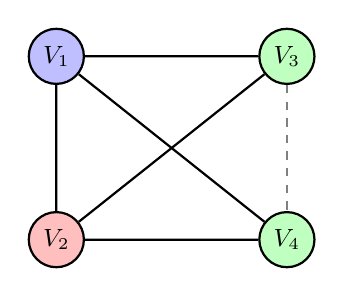
\begin{tikzpicture}[node distance=1.6cm]
    \node[vertex, fill=blue!25]  (v1) {$V_1$};
    \node[vertex, fill=red!25, below=of v1] (v2) {$V_2$};
    \node[vertex, fill=green!25, right=2.2cm of v1] (v3) {$V_3$};
    \node[vertex, fill=green!25, right=2.2cm of v2] (v4) {$V_4$};
    \draw[thick] (v1) -- (v2) (v1) -- (v3) (v1) -- (v4) (v2) -- (v3) (v2) -- (v4);
    \draw[thick, dashed, gray] (v3) -- (v4);
  \end{tikzpicture}
  \[
    \begin{aligned}
      \Enc[G_1 \Rightarrow LA(\mathbb{Z})] = {}&
        (c_1 = 1) \wedge (c_2 = 2) \wedge (c_3 = 3) \wedge
        \textstyle\bigwedge_{i=1}^{4} \big((v_i \geq 1) \wedge (v_i \leq 3)\big) \;\wedge \\
      & \neg(v_1 = v_2) \wedge \neg(v_1 = v_3) \wedge \neg(v_1 = v_4) \wedge
        \neg(v_2 = v_3) \wedge \neg(v_2 = v_4)
    \end{aligned}
  \]
  \caption{A 3-colorable graph $G_1$ (solid edges) with a valid coloring, and its
  encoding into linear integer arithmetic using the colorer of
  Example~\ref{ex:lia}. Adding the dashed edge $\langle V_3, V_4 \rangle$ gives a
  graph $G_2$ that is not 3-colorable, and adding $\neg(v_3 = v_4)$ makes the
  formula unsatisfiable (after~\cite[Fig.~1]{Sebastiani16}).}
  \label{fig:example}
\end{figure}

Two more results of the paper are important for us. First, \emph{every
$k$-colorable theory is non-convex}; therefore, convex theories such as EUF have
no $k$-colorer at all. Second, if the domain of $\T$ has exactly $k \geq 3$
elements, then $\AllDiff_k(c)$ alone is a $k$-colorer (since a $(k+1)$-th distinct
value cannot exist). This covers, for example, fixed-width bit-vectors of width
$w > 1$, with $k = 2^w$. Using these tools, the paper builds colorers for
fragments of integer and non-linear real arithmetic, bit-vectors, floating point,
lists (with $k = 4$, using only $\mathit{nil}$, $\mathit{cons}$, $\mathit{car}$ and
$\mathit{cdr}$), finite sets (using only $\subseteq$ and the set enumerator), and
arrays (a chain of three $\mathit{store}$ operations). It also extends the
definition to theories \emph{without} equality, where equality and disequality are
\emph{emulated} by other literals, and shows a theory with domain size $\geq 3$
that is NP-hard and non-convex but not $k$-colorable for any $k \geq 3$.

The paper ends with open directions, among them: extending colorers to use
uninterpreted symbols as auxiliary variables, overcoming the restriction to domain
size $\geq 3$ by encoding vertices and colors as \emph{pairs} of variables, and an
``extensive exploration of the pool of available NP-hard theories, proving the
$k$-colorability of as many theories/fragments as possible''. This last direction
is the starting point of our research.

\subsection{Graph Coloring with SAT and SMT}

Encoding graph coloring into SAT is a well-studied problem. Van
Gelder~\cite{VanGelder08} compares the direct encoding with the multivalued and
log encodings (one bit-vector of $\lceil \log_2 k \rceil$ bits per vertex) and with
the support encoding. Ramani et al.~\cite{RamaniAMS06} study symmetry breaking for
exact graph coloring, both by symmetry-breaking predicates that do not depend on the
instance (for example, fixing the colors of a clique) and by detecting the
symmetries of each instance. Hebrard and Katsirelos~\cite{HebrardK18} combine
clause learning with Zykov-style branching and coloring-specific bounds. These works
all target one encoding language (CNF) and one kind of solver.

On the SMT side, graph coloring appears mostly as an example. Of special interest
to us is the finite model finding procedure of Reynolds et al.~\cite{ReynoldsTGK13},
implemented in cvc5 as a $\T$-solver for EUF with \emph{cardinality constraints}.
To satisfy a constraint ``the sort $S$ has at most $k$ elements'', this solver must
merge the equivalence classes of $S$-terms down to $k$ without merging two classes
that are disequal; this is $k$-coloring of the disequality graph, and the solver
does it by splitting on merges, which corresponds to Zykov's
branching~\cite{Zykov49}. To the best of our knowledge, a systematic comparison of
graph coloring encodings across SMT theories and solvers has not been done.

% ===========================================================================
\section{Research Goal}
% ===========================================================================

The main research goal is ``\emph{Graph Coloring Modulo Theories}'', that is, to
study graph $k$-colorability as a single problem that can be expressed in (almost) every
SMT theory, both from the theoretical side, through $k$-colorers, and from the
practical side, through the behaviour of SMT-solvers on the resulting encodings.

Our motivation comes from three reasons:
\begin{enumerate}
  \item \textbf{Complexity of theories and fragments.} Knowing which theories and
    which fragments are NP-hard for $\T$-solving is not only of theoretical
    interest. As noted in~\cite{Sebastiani16}, it is important for SMT-solver
    development, since it decides how the search load should be split between the
    SAT-solver and the $\T$-solvers. Many theories that are supported by modern
    solvers, such as strings with regular expressions, bags, finite fields and
    separation logic, are not discussed in~\cite{Sebastiani16}. Finding $k$-colorers
    for small fragments of these theories pinpoints which constructs make them hard.
    For example, a colorer that uses only regular-expression membership shows that
    conjunctions of membership literals and disequalities between string variables
    are already NP-hard, without concatenation or length constraints.

  \item \textbf{Comparing theories and solvers.} A $k$-colorer is also an encoding
    of graph coloring that can be given to a solver. Since many theories have many
    different colorers, we obtain a family of formulas that all express the same
    combinatorial problem, on the same graphs, but exercise completely different
    $\T$-solvers (bit-blasting, simplex, non-linear arithmetic, string, set and
    cardinality solvers, Gr\"obner-basis reasoning for finite fields, and more).
    This makes it possible to ask questions that are hard to ask with
    the usual SMT-LIB benchmarks, which come from different sources for different
    theories. For example: Does being a $k$-colorer (that is, keeping the choice
    inside the $\T$-solver) make an encoding harder or easier than a disjunctive
    encoding? Which internal technique of the solver is responsible for the
    difference?

  \item \textbf{Better graph coloring with SMT.} The encodings expose solver
    techniques that are useful for graph coloring itself. One example is the
    cardinality solver of cvc5, which has no color symmetry and can therefore
    refute some instances that are hard for a SAT-based encoding (see
    Section~\ref{sec:prelim}). Understanding these effects can lead to
    preprocessing strategies and portfolios that combine the strengths of different
    encodings.
\end{enumerate}

% ===========================================================================
\section{Research Assumption}
% ===========================================================================

In our research we assume:
\begin{enumerate}
  \item Many theories supported by modern SMT-solvers are $k$-colorable for some
    $k \geq 3$ with very small fragments of their signature. This assumption is
    based on~\cite{Sebastiani16}, where colorers were found easily for many
    theories, and on our preliminary results, where we already found colorers for
    theories and fragments that are not covered by the paper.
  \item Different encodings of the same coloring problem lead to large differences
    in solver performance, and these differences can be explained by the internal
    techniques of the $\T$-solvers. This assumption is based on our preliminary
    results in Section~\ref{sec:prelim}.
\end{enumerate}

% ===========================================================================
\section{Research Plan}
% ===========================================================================

Our research plan is comprised of the following parts:

\begin{enumerate}
  \item \textbf{Build an infrastructure for graph coloring modulo theories.}
    We build a tool, which we call \tool{}, that reads a graph in the DIMACS
    format and a number $k$, builds an encoding of $k$-colorability in a chosen
    theory, solves it with a chosen solver and checks the returned coloring against
    the graph. The encodings are written against the native C++ APIs of cvc5 and Z3,
    with the same encoding names and output in both, so that the two solvers can be
    compared encoding by encoding. Encodings that do not depend on the type of their
    elements (for example, set membership or array chains) are parameterized by an
    \emph{element theory}, so that the same colorer can be run over integers,
    bit-vectors, strings, uninterpreted sorts and so on. The tool also includes a
    benchmarking script, a script that computes the chromatic numbers of the
    benchmark graphs, and a graphical interface that shows the asserted formulas in
    mathematical notation together with the resulting coloring. Most of this part
    is already done (see Section~\ref{sec:prelim}).

  \item \textbf{Find and prove new $k$-colorers.} For every theory supported by
    cvc5 and Z3, we will design encodings that satisfy Definition~\ref{def:colorer},
    prove that they are $k$-colorers, and derive the NP-hardness of the
    corresponding fragment. We will focus on theories and fragments that are not
    covered in~\cite{Sebastiani16}: strings (regular-expression membership,
    $\mathit{str.contains}$ with a constant word, lexicographic order),
    bags (sub-bag inclusion), finite fields (polynomials and roots of unity),
    separation logic, transcendental functions over the reals, and small
    bit-vector fragments (for example, only bit-wise \emph{and} or only shifts).
    Since a smaller fragment gives a stronger result, we will look for the smallest
    signature that still admits a colorer. For each encoding that is \emph{not} a
    colorer as written, we will determine whether this is a property of the
    encoding (and a colorer exists in the same theory) or of the theory.

  \item \textbf{Study the limits of colorability.} We will study the theories that
    cannot have a $k$-colorer: convex theories (by~\cite{Sebastiani16}, a
    $k$-colorable theory is non-convex), theories whose domain is too small, and
    encodings in which a vertex is represented by more than one variable (for
    example, a point in the plane), which corresponds to the ``pairs of variables''
    extension proposed in~\cite{Sebastiani16}. We will also consider the variant of
    the definition for theories without equality, where edges are emulated
    disequalities, since several of our encodings replace $\neg(u = v)$ with a
    theory-specific edge constraint.

  \item \textbf{Evaluate the encodings experimentally.} We will run all the encodings
    with cvc5 and Z3 on the DIMACS graph coloring benchmarks~\cite{JohnsonT96},
    each graph with $k = \chi(G)$ (satisfiable) and $k = \chi(G) - 1$
    (unsatisfiable), with every model checked. We will compare the encodings with
    each other, the two solvers with each other, and both with dedicated tools for
    graph coloring, such as the CP-SAT solver of OR-Tools~\cite{ortools} and
    the CDCL-based solver of~\cite{HebrardK18}. For every large difference in
    performance, we will try to find the responsible technique inside the solver
    (bit-blasting, non-linear real arithmetic, the cardinality solver, and so on).
    We will also check whether being a $k$-colorer is related to performance at all.

  \item \textbf{Improve solving.} Based on the experiments, we will develop
    techniques that improve SMT-based graph coloring. These include strategies that
    run on the graph before the solver and work with every encoding, such as fixing
    the colors of a clique to break the color symmetry, removing vertices that can
    always be colored afterwards, and answering easy instances with a heuristic; and
    encodings with no color symmetry at all, such as the cardinality encoding and
    encodings based on representatives. We will also evaluate a portfolio of
    encodings.

  \item (optional) \textbf{Contribute benchmarks.} Some theories, such as finite
    fields, bags and separation logic, have few benchmarks in SMT-LIB. We will
    generate families of benchmarks from the encodings, with known answers
    (since $\chi(G)$ is known), and propose them to the SMT-LIB benchmark
    library.

  \item (optional) \textbf{Use colorers to find solver issues.} Since all the
    encodings of the same instance must give the same answer, and every model can be
    checked against the graph, the framework is also a differential testing tool for
    SMT-solvers. We will report wrong answers, invalid models and
    \texttt{unknown} results that we find to the solver developers.
\end{enumerate}

% ===========================================================================
\section{Preliminary Results}\label{sec:prelim}
% ===========================================================================

So far we have built most of the infrastructure described in the first part of the
research plan. \tool{} currently has 51 encodings in cvc5, 13 of them
parameterized by an element theory and runnable over 9 element theories, and 36 of
them also in Z3 (Z3 does not support finite fields, bags, separation logic or
trigonometric functions). The four trigonometric encodings can also be solved by
dReal. An earlier version of the tool was built on top of
Smt-Switch~\cite{smtswitch}; we moved to the native APIs in order to use features
that are specific to one solver, such as cardinality constraints and finite fields.
Figure~\ref{fig:smtlib} shows two of the encodings.

\begin{figure}[t]
  \centering
  \begin{minipage}[t]{0.48\textwidth}
\begin{lstlisting}
(set-logic QF_BV)
(declare-const v1 (_ BitVec 2))
(declare-const v2 (_ BitVec 2))
(declare-const v3 (_ BitVec 2))
; domain: 1 <= v <= 3
(assert (bvule #b01 v1))
(assert (bvule v1 #b11))
...
; one disequality per edge
(assert (not (= v1 v2)))
(assert (not (= v1 v3)))
(assert (not (= v2 v3)))
(check-sat)
\end{lstlisting}
  \end{minipage}\hfill
  \begin{minipage}[t]{0.48\textwidth}
\begin{lstlisting}
(set-logic QF_UFC)
(declare-sort Color 0)
(declare-const v1 Color)
(declare-const v2 Color)
(declare-const v3 Color)
; no domain constraints
; one disequality per edge
(assert (not (= v1 v2)))
(assert (not (= v1 v3)))
(assert (not (= v2 v3)))
; the sort has at most K elements
(assert (_ fmf.card Color 3))
(check-sat)
\end{lstlisting}
  \end{minipage}
  \caption{3-coloring a triangle. Left: the \enc{BV} encoding, a $k$-colorer for
  fixed-width bit-vectors. Right: the \enc{UF-CARD} encoding, where a single
  cardinality constraint of cvc5 replaces all the domain constraints.}
  \label{fig:smtlib}
\end{figure}

\paragraph{Classification of the encodings.}
We checked every encoding against Definition~\ref{def:colorer}.
Table~\ref{tab:colorers} summarizes the result for the 49 encodings that existed at
the time of the classification. Among the colorers, several are for theories or
fragments that are not covered in~\cite{Sebastiani16}, for example:
\begin{itemize}
  \item \textbf{Strings}: $x \in (\texttt{"A"} \mid \texttt{"B"} \mid \dots)$, a
    single regular-expression membership literal; and
    $\mathit{str.contains}(W, x)$ for a constant word $W$ that has exactly $k$
    distinct substrings (the empty string included).
  \item \textbf{Bags}: $x \sqsubseteq \{e_1 : p_1 - 1, \dots, e_L : p_L - 1\}$, where
    $p_1 \cdots p_L = k$ is the prime factorization of $k$, so that the bag has
    exactly $k$ sub-bags.
  \item \textbf{Finite fields}: $x^k = 1$ in $GF(p)$ with $k \mid p - 1$ (the
    $k$-th roots of unity), and $x(x-1)\cdots(x-k+1) = 0$.
  \item \textbf{Bit-vectors}: the order encoding $(x \mathbin{\&} (x+1)) = 0$ over
    $k-1$ bits, and the same set of values stated without an adder,
    $((x \gg 1) \mathbin{\&} {\sim}x) = 0$.
  \item \textbf{Transcendental functions}: $\sin(x) = 0$ in a box that contains
    exactly $k$ roots.
\end{itemize}
The encodings that are not colorers fall into a few groups: encodings whose domain
is a disjunction (which is unavoidable for EUF, since it is convex), encodings with
no vertex variable at all (for example, one set of vertices per color, or a single
relation between vertices and colors), and encodings in which a vertex is
represented by several variables.

\begin{table}[t]
  \centering
  \small
  \begin{tabularx}{\textwidth}{@{}lcX@{}}
    \toprule
    Status & \# & Encodings \\
    \midrule
    $k$-colorer as written & 25 &
      \enc{LIA}, \enc{IDL}, \enc{BV}, \enc{BV-ZERO}, \enc{BV-AND},
      \enc{BV-ORDER}, \enc{BV-ORDER-SHIFT}, \enc{NLRA}, \enc{NLRA-SQRT}, four
      trigonometric, \enc{FF-POLY}, \enc{FF-ROOTS}, \enc{STR-LEX}, \enc{STR-INT},
      \enc{STR-REG}, \enc{STR-SUB}, \enc{ARR-EXP}, \enc{SET-CUBE},
      \enc{SET-MASK}, \enc{SET-MEM}, \enc{BAG-SUB}, \enc{BAG-UNARY} \\
    $k$-colorer after naming a term & 4 &
      \enc{INT-MOD}, \enc{INT-POW2}, \enc{BV-MOD}, \enc{ARR-INL} \\
    $k$-colorer by domain size & 2 &
      \enc{FF-PRIME}, \enc{UF-CARD} (cvc5) \\
    colorer domain, other edges & 4 &
      \enc{BV-ONEHOT}, \enc{FP}, \enc{FF-NULL}, \enc{SEP} \\
    not a $k$-colorer & 14 &
      \enc{NLRA-ROOTS}, \enc{UF}, \enc{LIST-UF}, \enc{LIST-DT}, \enc{PEANO},
      \enc{BOOL-DIRECT}, \enc{BOOL-DIRECT-AMO}, \enc{STRING}, \enc{ARR-MAP},
      \enc{SET-CLASSES}, \enc{REL-JOIN}, \enc{BAG-CARD}, \enc{BAG-NEIGHBORS},
      \enc{OR} \\
    \bottomrule
  \end{tabularx}
  \caption{Classification of the encodings according to
  Definition~\ref{def:colorer}. ``After naming a term'' means that the color of a
  vertex is a term over an auxiliary variable (such as $x \bmod k$), and naming
  this term $v_i$ gives a colorer. ``Other edges'' means that the vertex part is a
  colorer, but the edges are a theory-specific constraint instead of
  $\neg(u = v)$.}
  \label{tab:colorers}
\end{table}

\paragraph{cvc5 and Z3.}
We ran every encoding that both solvers support on three satisfiable and three
unsatisfiable instances (\texttt{myciel4}, \texttt{queen5\_5}, \texttt{DSJC125.1}
and \texttt{1-FullIns\_4}) with a timeout of 30 seconds, and checked every model.
Z3 solved 177 of the 216 runs and cvc5 solved 164. The differences between the
solvers are much larger than this total suggests, and they depend on the theory.
Z3 is much faster on non-linear real arithmetic (it solves 5 of 6 instances of the
polynomial encodings, while cvc5 times out on all of them), on floating point, on
the array chains, and on encodings that consist of equalities between constants.
cvc5 is faster on the encodings that use string operations, on difference logic and
on the Peano-numbers datatype encoding. On the bit-vector encodings and the direct
SAT encoding both solvers take well under a second, since both bit-blast to a SAT
solver. Our results also show that being a colorer is not related to performance in
an obvious way: among the fastest encodings are both colorers (\enc{BV},
\enc{BV-AND}, \enc{SET-MEM}) and non-colorers (\enc{BOOL-DIRECT}, \enc{UF},
\enc{OR}). A non-colorer moves the case split from the $\T$-solver into the
SAT-solver, which handles it very well.

\paragraph{The cardinality encoding.}
The \enc{UF-CARD} encoding (Figure~\ref{fig:smtlib}, right) has no colors at all:
the values of the vertices are anonymous elements of an uninterpreted sort, and the
cardinality solver of cvc5~\cite{ReynoldsTGK13} performs Zykov-style branching on
them. As a result, the search never revisits the $k!$ renamings of a coloring, and
a $(k+1)$-clique, which is a pigeonhole problem for a SAT-solver, is detected in one
step. On the complete graph $K_{k+1}$ with $k$ colors, \enc{UF-CARD} takes 0.12
seconds for every $k$ between 8 and 12, while the time of \enc{BV} grows from 0.22
to 11 seconds, and \enc{UF} times out from $k = 10$. On the DIMACS benchmarks it is
the fastest encoding on a family of hard unsatisfiable instances (the
\texttt{FullIns} graphs), and the only one that refutes \texttt{5-FullIns\_4} with
8 colors, while it is slower than \enc{BV} on almost every satisfiable instance.

\paragraph{Strategies.}
Following this observation, we implemented strategies that run on the graph before
the solver and work with every encoding: a DSATUR pre-check, the removal of
dominated vertices and of vertices with fewer than $k$ neighbours (which are
colored back afterwards), and fixing the colors of a large clique, which breaks the
color symmetry. Table~\ref{tab:strategies} shows the effect on all the 56 graphs
with a known chromatic number. With strategies, the \enc{BV} encoding solves all 112
instances, where it solved 93 without them, and the total time of the
unsatisfiable instances drops from 609 to 15 seconds.

\begin{table}[t]
  \centering
  \small
  \begin{tabular}{@{}llrrrr@{}}
    \toprule
    Encoding & Strategies & \multicolumn{2}{c}{SAT ($k = \chi$)} &
      \multicolumn{2}{c}{UNSAT ($k = \chi - 1$)} \\
    \cmidrule(lr){3-4}\cmidrule(lr){5-6}
     & & solved & time & solved & time \\
    \midrule
    \enc{BV}          & none                          & 55 & 144 s & 38 & 609 s \\
    \enc{BV}          & clique                        & 56 & 128 s & 56 &  60 s \\
    \enc{BV}          & dominated, peel, clique       & 56 & 102 s & 56 &  15 s \\
    \enc{BV}          & all four                      & 56 &  93 s & 56 &  15 s \\
    \enc{BOOL-DIRECT} & none                          & 56 & 110 s & 31 & 766 s \\
    \enc{BOOL-DIRECT} & dominated, peel, clique       & 56 &  37 s & 56 &  27 s \\
    \bottomrule
  \end{tabular}
  \caption{The effect of the graph strategies with cvc5 on the 56 DIMACS graphs with a
  known chromatic number, 30 seconds timeout (timeouts are counted as 30 seconds).}
  \label{tab:strategies}
\end{table}

Notice that while running these experiments the framework already found a
solver issue: an early translation of the relation-based encoding to Z3 used
existential quantifiers inside lambda terms, and on the complete graph $K_4$ Z3
returned a model in which two adjacent vertices have the same color. Replacing the
quantifier with a finite disjunction fixed the encoding. In order to finish the
first part of the research plan, we need to complete the documentation of the
encodings and to run the full experimental comparison on all the benchmarks.

\bibliographystyle{plain}
\bibliography{references}

\end{document}
